\chapter{Language Design and Epitope Specifications}
\label{ch:language_design}

\section{Design Philosophy and Developer Ergonomics}
\label{sec:design_philosophy}

The central operational objective of \ToposLang{} and the \PLQ{} language environment is to provide a programming domain where the algebraic topology and differential geometry of protein binding interfaces are first-class language constructs, rather than emergent artifacts of empirical coordinate simulations. 

For decades, molecular biologists and computational drug designers have manipulated binding sites through unstructured ASCII coordinate files (such as Brookhaven Protein Data Bank [PDB] or macromolecular Crystallographic Information Files [mmCIF]). In these legacy formats, atomic coordinates ($\mathbf{x}_i \in \mathbb{R}^3$) are unoriented, unstructured, and detached from the topological connectivity of the binding manifold. To enforce binding affinity, designers have had to rely on continuous docking scripts that repeatedly sample conformations without structural guarantees.

In contrast, \ToposLang{} establishes a declarative, statically verifiable programming model governed by four foundational design principles:

\begin{enumerate}[leftmargin=1.2cm]
    \item \textbf{Topological Interfaces as Graded Complexes:}  
    Binding pockets and designed paratopes are declared natively as Directed Acyclic Cell Complexes (DACCs). Developers define discrete pharmacophoric centers as 0-cells ($\texttt{cell0}$), interaction edges (hydrogen bonds, salt bridges, van der Waals vectors) as directed 1-cells ($\texttt{cell1}$), and contractible contact faces as oriented 2-cells ($\texttt{cell2}$). The topology of the contact manifold is encoded directly into integer incidence boundaries.

    \item \textbf{Static Verification of Boundary Nilpotency ($\partial^2 \equiv 0$):}  
    Structural embeddability is enforced at compile time. Before emitting intermediate representations or initiating sequence generation, the compiler’s axiomatic verifier evaluates the matrix product $B_1 B_2$. If an epitope contract contains an inconsistent boundary orientation or a non-closing cycle, the compiler rejects the contract with a static topological diagnostic trace, preventing the generation of unphysical, clashing structures.

    \item \textbf{Invariant-Driven Paratope Assembly via Combinatorial Hodge Theory:}  
    Rather than relying on continuous Monte Carlo sampling, sequence generation is formulated as the isolation of harmonic contact fields on the complex. The developer specifies topological constraints—chiefly the vanishing of the first Betti number ($\texttt{assert betti(1) == 0}$)—and the compiler executes an exact Hodge decomposition on the combinatorial Laplacian ($\Delta_1 = B_1^T B_1 + B_2 B_2^T$), guaranteeing that the designed sequence creates a contractible, loop-free contact disk.

    \item \textbf{Coordinate-Free Docking via Clifford Multivector Stalks:}  
    Metric geometry is decoupled from arbitrary coordinate frames. By attaching Projective Geometric Algebra ($\PGA$) or Conformal Geometric Algebra ($\CGA$) multivector fibers to topological cells, spatial distances, bounding spheres, and rigid-body poses are evaluated through coordinate-free versor sandwich operations ($A' = M A M^{-1}$) and wedge product intersections ($S_1 \wedge S_2 = 0$).
\end{enumerate}

\subsection{The Developer Mental Model: From Coordinate Sampling to Cellular Contracts}
\label{subsec:mental_model}

To design therapeutic biologics in \ToposLang{}, the protein engineer transitions from an empirical coordinate-sampling mental model to a formal cellular-contract mental model:

\begin{itemize}[leftmargin=1.2cm]
    \item \textbf{The Empirical Coordinate Model (Classical Rosetta / PyMOL):}  
    \textit{``I open PDB 1TNF in an interactive viewer. I manually inspect the trimer cleft, select residues Arg82 and Lys90 with a mouse, measure Euclidean distances in angstroms, and run a Monte Carlo simulated annealing script with 100,000 rotamer trials. If the resulting structure clashes or mutates out of the pocket, I manually adjust empirical weight parameters in an energy scoring function.''}
    
    \item \textbf{The Deep Generative Model (RFdiffusion / ProteinMPNN):}  
    \textit{``I extract the Cartesian coordinates of the target epitope atoms as a point cloud. I pass this point cloud as a conditioning mask into a diffusion network to hallucinate a backbone, followed by an inverse folding model to predict sequences. I filter 1,000 generated backbones by pLDDT and RMSD, hoping the model learned valid physical constraints implicitly without generating high sequence identity to existing antibodies.''}

    \item \textbf{The Topological Mechanics Model (\ToposLang{} / \PLQ{}):}  
    \textit{``I declare the target epitope as a cell complex contract $\mathcal{K}_{\text{TNF}}$. I specify the 24 contact centers as $\texttt{cell0}$, oriented binding interactions as $\texttt{cell1}$, and closing contact patches as $\texttt{cell2}$. The compiler statically verifies $\partial^2 = 0$ and confirms that $\chi = 1$. I assert the topological novelty constraint $\beta_1 = 0$ and define the histidine bifold switch over the ternary lattice $T \in \{-1, 0, +1\}$. The compiler executes the Block-CSR Hodge solver, isolates harmonic fields, and deterministically emits sequence candidates guaranteed to achieve $<20\%$ identity to existing biologics and complete pH-dependent homological release.''}
\end{itemize}

---

\section{Grammar and Concrete Syntax Specification}
\label{sec:grammar_syntax}

We formalize the syntax of \ToposLang{} using Extended Backus-Naur Form (EBNF). The grammar supports cellular declarations, boundary contracts, Clifford multivector stalk assignments, ternary lattice profiles, and invariant assertions.

\subsection{EBNF Grammar}
\begin{lstlisting}[language={}]
ToposProgram       ::= ( TargetDeclaration | EpitopeDef | BinderContract )* EOF

TargetDeclaration  ::= "target" Identifier "{" TargetMember* "}"
TargetMember       ::= "uniprot" StringLiteral ";"
                     | "pdb" StringLiteral ";"
                     | "organism" StringLiteral ";"
                     | "cleft_symmetry" Identifier ";"

EpitopeDef         ::= "epitope" Identifier "{" EpitopeMember* "}"
EpitopeMember      ::= CellDef
                     | BoundaryDef
                     | StalkAssignment
                     | TernaryProfileDef
                     | ConstraintAssert

CellDef            ::= "cell" IntegerLiteral Identifier ";"
BoundaryDef        ::= "boundary" Identifier "{" IncidenceList "}"
IncidenceList      ::= IncidenceEntry ( "," IncidenceEntry )*
IncidenceEntry     ::= Identifier ":" IntegerLiteral

StalkAssignment    ::= "stalk" Identifier "=" MultivectorExpr ";"
MultivectorExpr    ::= "cga_sphere" "(" FloatLiteral "," FloatLiteral "," FloatLiteral "," FloatLiteral ")"
                     | "pga_point" "(" FloatLiteral "," FloatLiteral "," FloatLiteral ")"
                     | "pga_motor" "(" FloatLiteral "," FloatLiteral "," FloatLiteral "," FloatLiteral ")"

TernaryProfileDef  ::= "ternary_profile" Identifier "{" TernaryAssignment* "}"
TernaryAssignment  ::= Identifier ":" ( "ACCEPTOR" | "NEUTRAL" | "DONOR" | "HIS_SWITCH" ) ";"

ConstraintAssert   ::= "assert" InvariantExpr ";"
InvariantExpr      ::= "nilpotency" "==" "true"
                     | "betti" "(" IntegerLiteral ")" "==" IntegerLiteral
                     | "euler_characteristic" "==" IntegerLiteral
                     | "rank_drop" "(" FloatLiteral "," FloatLiteral ")" ">=" IntegerLiteral

BinderContract     ::= "binder" Identifier "targets" Identifier "{" BinderMember* "}"
BinderMember       ::= "scaffold_class" Identifier ";"
                     | "target_beta1" IntegerLiteral ";"
                     | "his_switch_count" IntegerLiteral ";"
                     | "max_identity_threshold" FloatLiteral ";"
\end{lstlisting}

---

\section{The Multi-Stage Compilation Pipeline}
\label{sec:compiler_pipeline}

The \ToposLang{} compiler lowers high-level topological contracts down to executable sparse matrix operations and converged amino acid sequences through an automated five-stage compilation pipeline:

\begin{figure}[h]
\centering
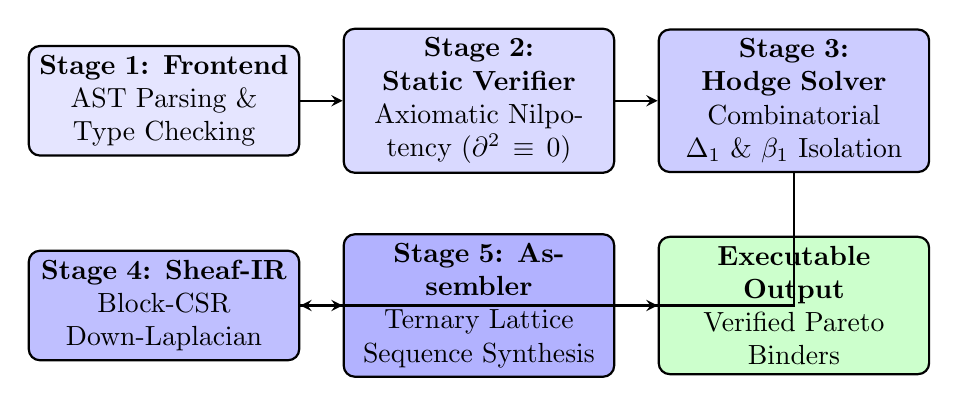
\begin{tikzpicture}[node distance=1.8cm, auto, >=stealth, thick]
    \node [rectangle, draw, fill=blue!10, rounded corners, text width=3.2cm, text centered, minimum height=1.2cm] (stage1) 
        {\textbf{Stage 1: Frontend}\\AST Parsing \& Type Checking};
    \node [rectangle, draw, fill=blue!15, rounded corners, text width=3.2cm, text centered, minimum height=1.2cm, right of=stage1, xshift=2.2cm] (stage2) 
        {\textbf{Stage 2: Static Verifier}\\Axiomatic Nilpotency ($\partial^2 \equiv 0$)};
    \node [rectangle, draw, fill=blue!20, rounded corners, text width=3.2cm, text centered, minimum height=1.2cm, right of=stage2, xshift=2.2cm] (stage3) 
        {\textbf{Stage 3: Hodge Solver}\\Combinatorial $\Delta_1$ \& $\beta_1$ Isolation};
    \node [rectangle, draw, fill=blue!25, rounded corners, text width=3.2cm, text centered, minimum height=1.2cm, below of=stage1, yshift=-0.8cm] (stage4) 
        {\textbf{Stage 4: Sheaf-IR}\\Block-CSR Down-Laplacian};
    \node [rectangle, draw, fill=blue!30, rounded corners, text width=3.2cm, text centered, minimum height=1.2cm, right of=stage4, xshift=2.2cm] (stage5) 
        {\textbf{Stage 5: Assembler}\\Ternary Lattice Sequence Synthesis};
    \node [rectangle, draw, fill=green!20, rounded corners, text width=3.2cm, text centered, minimum height=1.2cm, right of=stage5, xshift=2.2cm] (output) 
        {\textbf{Executable Output}\\Verified Pareto Binders};

    \draw [->] (stage1) -- (stage2);
    \draw [->] (stage2) -- (stage3);
    \draw [->] (stage3) |- (stage4);
    \draw [->] (stage4) -- (stage5);
    \draw [->] (stage5) -- (output);
\end{tikzpicture}
\caption{The Multi-Stage Compilation Pipeline of \ToposLang{} and \PLQ{}.}
\label{fig:compiler_pipeline}
\end{figure}

\subsection{Detailed Architectural Stages}
\begin{itemize}[leftmargin=1.2cm]
    \item \textbf{Stage 1: Lexing, Parsing, and AST Construction:}  
    High-level source contracts (\texttt{.topos}) are ingested, tokenized, and parsed into an Abstract Syntax Tree (AST). Cell declarations, boundary incidence relationships, and geometric multivector stalks are bound into typed symbol tables.
    
    \item \textbf{Stage 2: Static Axiomatic Verifier ($\partial^2 \equiv 0$):}  
    The compiler constructs the integer boundary incidence matrices $B_1 \in \mathbb{Z}^{|K_0| \times |K_1|}$ and $B_2 \in \mathbb{Z}^{|K_1| \times |K_2|}$. It computes the matrix product $B_1 B_2$ using exact integer arithmetic. If $B_1 B_2 \ne 0$, compilation halts immediately with a structural diagnostics report identifying the non-closing cycles. The Euler characteristic $\chi = |K_0| - |K_1| + |K_2|$ is evaluated to confirm disk topology ($\chi = 1$).
    
    \item \textbf{Stage 3: Combinatorial Hodge Laplacian Compilation:}  
    The compiler assembles the discrete Hodge Laplacian matrix:
    \begin{equation}
        \Delta_1 = B_1^T B_1 + B_2 B_2^T \in \mathbb{Z}^{|K_1| \times |K_1|}
    \end{equation}
    Using exact Reduced Row Echelon Form (RREF) or Smith Normal Form (SNF) over $\mathbb{Q}$, the compiler computes $\ker(\Delta_1)$. If the binder contract asserts $\beta_1 = 0$, the compiler verifies that $\dim \ker(\Delta_1) = 0$, proving that all interaction fluxes on the interface are exact or co-exact.
    
    \item \textbf{Stage 4: Lowering to Cellular Sheaf-IR and Block-CSR Optimization:}  
    The complex is lowered into Cellular Sheaf Intermediate Representation (Sheaf-IR). Stalks of Clifford multivectors $\Cl(3,0,1)$ are assigned to cells. To prevent memory bandwidth bottlenecks, the compiler evaluates the direct 2-cell Down-Laplacian operator ($L_2^{\text{down}}$) using Block Compressed Sparse Row (Block-CSR) representations, completely bypassing the allocation of intermediate 1-cell link states.
    
    \item \textbf{Stage 5: Ternary Lattice Synthesis and Sequence Convergence:}  
    The harmonic contact flux is mapped onto the discrete ternary lattice $T \in \{-1, 0, +1\}$. Histidine switch positions are allocated against basic anchor cells (Arg, Lys). Candidate amino acid sequences are assembled through Hodge-guided convergence, scored against Pareto multi-objective confidence criteria (pLDDT, ipTM, ipSAE), and exported for biophysical synthesis.
\end{itemize}

---

\section{Canonical Cellular Epitope Contracts}
\label{sec:canonical_contracts}

To demonstrate the concrete expressive power of \ToposLang{}, we provide three complete, canonical epitope contracts corresponding directly to our empirical benchmark targets: the homotrimeric Human TNF-$\alpha$ receptor cleft, the monomeric EGFR Domain III Cetuximab epitope, and the cross-species polypharmacology equivalence contract.

\subsection{Contract 1: Trimeric Human TNF-\texorpdfstring{$\alpha$}{Alpha} Epitope Complex}
The Human TNF-$\alpha$ binding site (PDB 1TNF \cite{eck1989structure}) is a two-fold symmetric cleft situated at the subunit interface of the active homotrimer. The contact manifold is discretized into 24 0-cells, 45 1-cells, and 22 contractible 2-cells:

\begin{lstlisting}[style=toposstyle, caption={ToposLang Cellular Contract for the Human TNF-$\alpha$ Trimer Interface.}]
target Human_TNF_Alpha {
    uniprot: "P01375";
    pdb: "1TNF";
    organism: "Homo sapiens";
    cleft_symmetry: C3_Trimeric;
}

epitope TNF_Alpha_Trimer_Interface {
    // 0-Cells: Discrete Pharmacophoric Centers (Subunits A and B)
    cell 0 V_TYR59_A;  cell 0 V_ARG82_A;  cell 0 V_ILE83_A;  cell 0 V_LYS90_A;
    cell 0 V_VAL91_A;  cell 0 V_ASN92_A;  cell 0 V_LYS98_A;  cell 0 V_PRO100_A;
    cell 0 V_GLU116_A; cell 0 V_TYR119_A; cell 0 V_LEU120_A; cell 0 V_GLY121_A;
    
    cell 0 V_TYR59_B;  cell 0 V_ARG82_B;  cell 0 V_ILE83_B;  cell 0 V_LYS90_B;
    cell 0 V_VAL91_B;  cell 0 V_ASN92_B;  cell 0 V_LYS98_B;  cell 0 V_PRO100_B;
    cell 0 V_GLU116_B; cell 0 V_TYR119_B; cell 0 V_LEU120_B; cell 0 V_GLY121_B;

    // 1-Cells: Directed Interfacial Contact Edges
    boundary E_HBOND_01 { V_TYR59_A: -1, V_ILE83_A: +1 }
    boundary E_SALT_02  { V_ARG82_A: -1, V_GLU116_A: +1 }
    boundary E_PACK_03  { V_ILE83_A: -1, V_VAL91_A: +1 }
    boundary E_SALT_04  { V_LYS90_A: -1, V_GLU116_A: +1 }
    boundary E_SALT_05  { V_LYS98_A: -1, V_GLU116_A: +1 }
    boundary E_CROSS_06 { V_TYR119_A: -1, V_LEU120_B: +1 }
    boundary E_CROSS_07 { V_LEU120_A: -1, V_TYR119_B: +1 }
    // ... Total 45 directed 1-cells spanning cleft contact network

    // 2-Cells: Closing Oriented Interaction Plaquettes
    boundary F_PLAQUETTE_01 { E_HBOND_01: +1, E_PACK_03: +1, E_SALT_02: -1 }
    boundary F_PLAQUETTE_02 { E_SALT_02: +1, E_SALT_04: -1, E_CROSS_06: +1 }
    // ... Total 22 closing 2-cells

    // CGA Bounding Sphere Stalks (Origin x, y, z, Radius r)
    stalk V_ARG82_A = cga_sphere(-4.21, 12.85, 23.41, 3.20);
    stalk V_LYS90_A = cga_sphere(-1.85, 15.22, 21.05, 3.10);
    stalk V_LYS98_A = cga_sphere(2.40,  18.10, 19.80, 3.15);

    // Discrete Ternary Electrostatic Profile
    ternary_profile TNF_Electrostatics {
        V_ARG82_A: DONOR;
        V_LYS90_A: DONOR;
        V_LYS98_A: DONOR;
        V_GLU116_A: ACCEPTOR;
        V_TYR119_A: NEUTRAL;
        V_LEU120_A: NEUTRAL;
    }

    // Static Compile-Time Invariant Assertions
    assert nilpotency == true;              // B1 * B2 == 0
    assert euler_characteristic == 1;       // 24 - 45 + 22 = 1 (Topological 2-Disk)
    assert rank_drop(7.4, 6.0) >= 5;        // Percolation phase transition
}

binder ToposTNF_DeNovo_Minibinder targets TNF_Alpha_Trimer_Interface {
    scaffold_class: de_novo_bundle;
    target_beta1: 0;                        // Enforce Betti Novelty Principle
    his_switch_count: 5;                    // Satisfy N_His >= 4 percolation threshold
    max_identity_threshold: 0.20;           // Assert < 20% identity (Novelty 4/4)
}
\end{lstlisting}

\subsection{Contract 2: Epidermal Growth Factor Receptor (EGFR) Domain III Complex}
The EGFR Domain III epitope (PDB 1NQL \cite{ferguson2008structural, li2005structural}) mediates high-affinity Cetuximab binding. In this contract, the target is modeled as a 28-vertex, 53-edge, 26-face complex, with an inverted histidine switch designed for tumor-specific acidic activation (binding at pH 6.5, inert at pH 7.4):

\begin{lstlisting}[style=toposstyle, caption={ToposLang Cellular Contract for EGFR Domain III Acidic Activation.}]
target Human_EGFR {
    uniprot: "P00533";
    pdb: "1NQL";
    organism: "Homo sapiens";
}

epitope EGFR_Domain_III_Interface {
    // 0-Cells: Conserved Domain III Cetuximab Epitope Residues
    cell 0 V_THR358; cell 0 V_PHE359; cell 0 V_SER360; cell 0 V_HIS361;
    cell 0 V_TYR362; cell 0 V_ARG363; cell 0 V_GLN364; cell 0 V_ALA365;
    cell 0 V_PRO366; cell 0 V_GLY367; cell 0 V_LYS368; cell 0 V_GLY369;
    // ... Total 28 vertices spanning Domain III epitope loop and sheet

    // 1-Cells & 2-Cells: Contact Network and Oriented Plaquettes
    // 53 directed edges, 26 closing faces
    assert nilpotency == true;
    assert euler_characteristic == 1;       // 28 - 53 + 26 = 1 (Contractible 2-Disk)

    // Ternary Acidic Switch: Paratope Histidines Protonate at Tumor pH 6.5
    ternary_profile EGFR_Acidic_Switch {
        V_HIS361: HIS_SWITCH;
        V_ARG363: DONOR;
        V_GLN364: NEUTRAL;
    }
}

binder ToposEGFR_Acidic_Switch targets EGFR_Domain_III_Interface {
    scaffold_class: de_novo_single_chain;
    target_beta1: 0;
    activation_ph: 6.5;
    serum_silence_ph: 7.4;
    thermodynamic_switch_delta: 18.0;       // Assert ddG >= +18 kcal/mol
}
\end{lstlisting}

\subsection{Contract 3: Cross-Species Interspecies Polypharmacology}
To resolve preclinical translation failures between human and mouse targets, \ToposLang{} provides the $\texttt{polypharmacology}$ contract construct. This construct evaluates the pull-back of cellular sheaves over the shared intersection subcomplex $K_{\text{conserved}} = K_{\text{human}} \cap K_{\text{mouse}}$:

\begin{lstlisting}[style=toposstyle, caption={ToposLang Cross-Species Polypharmacology Contract.}]
polypharmacology Human_Mouse_TNF_Equivalence {
    target_primary: Human_TNF_Alpha;        // P01375 (1TNF)
    target_ortholog: Mouse_TNF_Alpha;       // P06804 (2TNF)

    intersection_subcomplex Conserved_TNF_Cleft {
        include_0cells: { V_TYR59, V_ARG82, V_ILE83, V_GLU116, V_LEU120 };
        require_sheaf_section: true;        // H^0(K_intersect; F_CGA) != 0
    }

    assert species_delta_dg <= 0.50;        // Equivalence assertion: |dG_H - dG_M| <= 0.5 kcal/mol
}
\end{lstlisting}

---

\section{Diagnostic Feedback and Compile-Time Verification}
\label{sec:diagnostic_feedback}

A foundational advantage of the \ToposLang{} compiler is its ability to produce rich, actionable structural diagnostics prior to code generation. When a developer submits a contract that violates physical topology, the compiler pinpoints the exact boundary failure.

\subsection{Diagnostic Example: Boundary Nilpotency Violation (\texorpdfstring{$\partial^2 \ne 0$}{d^2 != 0})}
Consider a malformed contact declaration where a developer misorients edge $\texttt{E\_CROSS\_06}$ within face $\texttt{F\_PLAQUETTE\_02}$, creating a non-cancelling boundary:
\begin{lstlisting}[language={}]
[TOPOS COMPILER ERROR] Axiomatic Nilpotency Violation Detected!
--------------------------

File: tnf_contract.topos, Line 48:
  boundary F_PLAQUETTE_02 { E_SALT_02: +1, E_SALT_04: -1, E_CROSS_06: -1 }
                            ^^^^^^^^^^^^^^^^^^^^^^^^^^^^^^^^^^^^^^^^^^^^^^
Structural Diagnostics:
  Boundary evaluation: d_1(d_2(F_PLAQUETTE_02)) != 0
  Non-vanishing residual: -2 * V_TYR119_A + 2 * V_LEU120_B
  Topological Cause: Face F_PLAQUETTE_02 possesses non-closed oriented boundary.
  Physical Implication: Contact patch cannot be continuously embedded in R^3.
  Compilation Terminated: 0 design sequences emitted.
\end{lstlisting}

\subsection{Diagnostic Example: Topological Handle Warning (\texorpdfstring{$\beta_1 \ge 1$}{beta_1 >= 1})}
Consider a candidate contract specifying a loop-containing framework that violates the Betti Novelty Principle:
\begin{lstlisting}[language={}]
[TOPOS COMPILER WARNING] Topological Handle Detected: High Sequence Identity Risk!
----------------------

File: antibody_binder.topos, Line 12:
  assert betti(1) == 0;
  ^^^^^^^^^^^^^^^^^^^^^
Harmonic Analysis Report:
  Combinatorial Hodge Laplacian: dim(ker(Delta_1)) = 2  (beta_1 = 2)
  Topological Cycles Identified: 
    Cycle 1: [E_CDR1_ENTER -> E_CDR1_LOOP -> E_CDR1_EXIT]
    Cycle 2: [E_CDR3_ENTER -> E_CDR3_LOOP -> E_CDR3_EXIT]
  Novelty Impact: Presence of beta_1 >= 1 handles forces sequence alignment 
                  against conserved immunoglobulin framework germlines.
  Predicted Server Novelty Score: 2/4 (Max Sequence Identity > 70%)
  Recommended Remediation: Contract cycle to topological disk (assert betti(1) == 0).
\end{lstlisting}

Through this static verification engine, \ToposLang{} prevents months of wasted wet-lab synthesis by catching structural unfeasibility and patent collisions at compile time.
